% Taxot — IEEE-style project report (NLP course project, Industry Track)
% Build:  cd docs/report && tectonic taxot_ieee_report.tex
\documentclass[conference]{IEEEtran}
\IEEEoverridecommandlockouts
\usepackage[T1]{fontenc}
\usepackage{cite}
\usepackage{amsmath,amssymb}
\usepackage{graphicx}
\usepackage{booktabs}
\usepackage{multirow}
\usepackage{array}
\usepackage{xcolor}
\usepackage{tikz}
\usetikzlibrary{arrows.meta,positioning,fit,backgrounds,calc}
\usepackage{pgfplots}
\pgfplotsset{compat=1.17}
\usepackage[hidelinks]{hyperref}
\usepackage{url}
\graphicspath{{../figures/}}

\definecolor{teal}{HTML}{0F766E}
\definecolor{tealsoft}{HTML}{CCFBF1}
\definecolor{amber}{HTML}{B45309}
\definecolor{ambersoft}{HTML}{FEF3C7}
\definecolor{greybar}{HTML}{A1A1AA}
\definecolor{redbar}{HTML}{B91C1C}
\newcommand{\rupee}{Rs.\,}

% ---------------------------------------------------------------- held-out test numbers
% (experiments/results_test.json, run once with the frozen C6 code)
% Numbers from experiments/results_test.json (held-out test, 123 questions, run 26 Nov 2026),
% docs/battery_before.json / docs/battery_after.json and experiments/load_test.json.
\newcommand{\TestRfive}{0.904}
\newcommand{\TestMRR}{0.822}
\newcommand{\TestOOS}{84.6\%$^\ddagger$}
\newcommand{\TestCalc}{100\%}
\newcommand{\TestRows}{%
B1 & 0.839 & 0.722 & 0.725 & 0.889 & 0.959 & 1.00 \\
C1 & 0.847 & 0.747 & 0.750 & 0.833 & 0.959 & 1.00 \\
C2 & 0.877 & 0.766 & 0.767 & 0.944 & 0.959 & 1.00 \\
C3 & 0.888 & 0.770 & 0.784 & 0.833 & 0.951 & 1.00 \\
C4 & 0.888 & 0.805 & 0.802 & \textbf{1.000} & 0.951 & 1.00 \\
C5 & 0.897 & 0.808 & 0.807 & \textbf{1.000} & 0.959 & 1.00 \\
\textbf{C6} & \textbf{0.904} & \textbf{0.822} & \textbf{0.819} & \textbf{1.000} & \textbf{0.959} & 1.00 \\
}
\newcommand{\TestDiscussion}{%
The final configuration generalises: C6 is again the best on every ranking metric (Recall@5 0.904 vs 0.917
on dev; MRR 0.822 vs 0.830), period accuracy stays at 1.000 on the 18 test time traps, and the calculator is
exact on all 13 test calculations. The ladder keeps its shape---fusion beats either retriever and the date
filter fixes period errors (C3 0.833 $\to$ C4 1.000)---with one difference: on test, letting the reranker
reorder (C3) did not hurt ranking (MRR 0.766 $\to$ 0.770), so the dev finding that reordering is harmful is
weaker than it looked on 53 questions. Per category, Recall@5 is 1.00 for GST and Hinglish, 0.96 for income
tax and 0.94 for time traps, but only 0.38 for calculations (the explanation passages retrieved are often
not the gold ones; the computed numbers are unaffected).

\textbf{One target is missed on test.} Out-of-scope refusal is 84.6\% (11/13), below the 90\% target that dev
(100\%, 5/5) appeared to meet. Both misses are GST enforcement or evasion questions phrased like ordinary
GST questions (a search and seizure under section~67; splitting a shop's sales between spouses to stay under
the registration threshold), which the intent classifier labels \emph{question} and the gate passes because
GST passages score well. Three answerable questions were wrongly refused (false-refusal rate 2.7\%), e.g.\
``My client paid my invoice but kept back 10\%. Why?''. Both are classifier errors, and the fix---more
enforcement and evasion examples in the intent training data, and a topic rule for ``search'', ``seizure'' and
``split sales''---must be validated on new questions, since the test set has now been used.}
\newcommand{\RobustText}{%
Before the real-question fixes, the battery passed 61/80 real and 12/28 hard cases; with the final code it
passes 69/80 and 24/28. The remaining failures are mostly intent errors at the edges: foreign-currency
salary phrased as ``\$3000 per month from a US client'', implicit amounts (``my wife earns 25k pm''), a
Hinglish monthly figure (``mera mahine ka 40 hazaar hai''), and procedural questions about the 2025 Act
classified as out of scope.}
\newcommand{\PerfText}{%
With a single user, the C6 pipeline without the writer (scrub, normalisation, intent, period, hybrid
retrieval, cross-encoder gate, calculator, citation check) takes p50 2.2\,s and p95 2.9\,s per question on a
laptop CPU; the hosted writer adds about 6\,s (end-to-end p50 8.1\,s, p95 18.3\,s on dev). Under 10 concurrent
users the throughput does not rise (0.45 $\to$ 0.37 questions/s) and p50 grows to 25\,s: the cross-encoder
saturates the CPU, so concurrency needs a GPU, a smaller or quantised gate model, or more replicas. The writer
uses about 730 input and 450 output tokens per answer (73k and 45k per 100 queries), which costs nothing on the
free tiers used; the cost per 100 queries at paid rates depends on the provider chosen.}


\begin{document}

\title{Taxot: A Period-Aware, Citation-Grounded\\Retrieval-Augmented Assistant for Indian\\Income Tax and GST in English and Hinglish}

\author{
\IEEEauthorblockN{Ritesh Patil}
\IEEEauthorblockA{B.Tech.\ in CSAI, Roll No.\ 230056\\Rishihood University}
\and
\IEEEauthorblockN{Meghavi Rao}
\IEEEauthorblockA{B.Tech.\ in CSAI, Roll No.\ 230044\\Rishihood University}
\and
\IEEEauthorblockN{Harshal Nerpagar}
\IEEEauthorblockA{B.Tech.\ in CSAI, Roll No.\ 230076\\Rishihood University}
\thanks{Natural Language Processing course project (Industry Track), November 2026. Code, data card, experiment logs and the live demo are in the project repository.}
}

\maketitle

\begin{abstract}
Indian taxpayers pay chartered accountants (CAs) to answer routine questions, and two recent law changes
made this worse: the Income-tax Act, 2025, in force from 1~April~2026 with a single ``Tax Year'', and the
GST rate rationalisation (``GST~2.0'') of 22~September~2025. A general-purpose large language model (LLM)
cannot tell which law applies to which period, does not cite its sources, and makes arithmetic errors. We
present \emph{Taxot}, a retrieval-augmented question-answering system that accepts English and romanised
Hindi--English (Hinglish), attaches a verifiable, dated citation to every claim, extracts the period a
question refers to and filters the knowledge base to the law in force for that period, abstains and
escalates to a CA when a question is out of scope or evidence is weak, and delegates all tax computation to
a deterministic, unit-tested calculator. The retriever fuses BM25 and multilingual-E5 rankings with
Reciprocal Rank Fusion and uses a cross-encoder only as a confidence gate. We evaluate an eight-step
ablation ladder (B0--C6) on a 176-question gold set with a leakage-controlled 30/70 split. On the
development set the final configuration reaches Recall@5 0.917 and MRR 0.830, answers every time-sensitive
question from the correct period, refuses all out-of-scope questions with 2.1\% false refusals, computes
tax with 100\% exact match, and raises key-fact accuracy from 10.4\% (the same LLM without retrieval) to
68.8\% with a 3B local model and 79.2\% with a hosted writer, with every citation valid. On the untouched
123-question test set it reaches Recall@5 \TestRfive{} and MRR \TestMRR{} with 100\% period accuracy and an
exact calculator, while out-of-scope refusal falls to 84.6\%, below its 90\% target. We also report a real-world check
on 80 public questions, a robustness battery, a deployed prototype, and an agentic extension that turns
answers into completed tax tasks.
\end{abstract}

\begin{IEEEkeywords}
retrieval-augmented generation, legal question answering, temporal reasoning, code-mixed text, Hinglish,
abstention, citation verification, tax law
\end{IEEEkeywords}

% =====================================================================================
\section{Introduction}

India has about 8.5~crore individual income-tax payers and 1.67~crore active GST registrations
(sources in the M1 problem brief). Most of their questions are routine---which regime to choose, which
deductions apply, which ITR form to file, whether GST registration is needed---yet answering them usually
means paying a CA or trusting unsourced online content.

Tax question answering is a demanding NLP testbed for three reasons:
\begin{enumerate}
\item \textbf{The answer depends on the period.} From 1~April~2026 the Income-tax Act, 2025 replaces the 1961
Act; GST rates moved to a 5\%/18\%/40\% structure on 22~September~2025. The same question has different correct
answers for different dates, a known weakness of QA systems~\cite{zhang2021situatedqa,chen2021timeqa}.
\item \textbf{Fluent wrong answers are costly.} Even commercial legal RAG tools hallucinate on 17--33\% of
queries~\cite{magesh2025hallucination}.
\item \textbf{Users code-mix.} Many write Hinglish (``80C mein kitna milta hai?''), where standard models
underperform~\cite{khanuja2020gluecos}.
\end{enumerate}

\textbf{Contributions.} (1)~A period-aware RAG pipeline: symbolic period extraction plus an
interval-overlap filter over chunk-level effective dates, with \emph{period substitution} that swaps in the
in-period version of a rule. (2)~A safety layer suited to a small generator: intent classification and a
reranker-score gate for abstention, post-hoc citation validation with numeric-faithfulness checks and an
extractive fallback, PII scrubbing, and a mandatory disclaimer. (3)~A deterministic calculator for both tax
regimes across three tax years; the LLM explains but never computes. (4)~An evaluation protocol with targets
fixed before building, a leakage-controlled split, and an ablation ladder that isolates each component,
plus a real-question check and a robustness battery. (5)~A deployed prototype and an agentic extension.

% =====================================================================================
\section{Related Work}

\textbf{Retrieval.} BM25~\cite{robertson2009bm25} remains a strong lexical baseline; dense dual
encoders~\cite{karpukhin2020dpr} and contrastively pre-trained embeddings such as
E5/mE5~\cite{wang2022e5,wang2024me5} capture paraphrase; BGE-M3~\cite{chen2024m3} unifies dense and sparse
signals. Reciprocal Rank Fusion (RRF)~\cite{cormack2009rrf} merges rankings without score calibration.
Cross-encoder rerankers~\cite{nogueira2019passage} trade compute for precision on a short candidate list.

\textbf{RAG and attribution.} RAG~\cite{lewis2020rag} provides provenance and an updatable memory. ALCE~\cite{gao2023alce}
and Liu et al.~\cite{liu2023verifiability} show that LLM citations are often incomplete or unsupported;
RAGAS~\cite{es2024ragas} evaluates faithfulness without references.

\textbf{Legal NLP.} CaseHOLD~\cite{zheng2021casehold}, ILDC~\cite{malik2021ildc} and
LegalBench-RAG~\cite{pipitone2024legalbenchrag} benchmark legal reasoning and retrieval; Magesh et
al.~\cite{magesh2025hallucination} measure hallucination in deployed legal RAG.

\textbf{Time, code-mixing, abstention and tools.} SituatedQA~\cite{zhang2021situatedqa} and
TimeQA~\cite{chen2021timeqa} show temporal brittleness. GLUECoS~\cite{khanuja2020gluecos} and
LinCE~\cite{aguilar2020lince} benchmark Hindi--English code-switching. Kamath et al.~\cite{kamath2020selective}
study selective QA. PAL~\cite{gao2023pal} and Toolformer~\cite{schick2023toolformer} show that LLMs should
delegate arithmetic to tools; ReAct~\cite{yao2023react} interleaves reasoning and tool use.

\textbf{Gap.} We found no open system that combines period-aware retrieval, Hinglish input, citation
validation, abstention and deterministic computation for Indian tax law, nor a public Indian tax-QA
benchmark.

% =====================================================================================
\section{Problem Definition and Business Case (M1)}

\textbf{Task.} Given a question $q$ in English or Hinglish and an explicit or implicit period, return
(a)~a grounded answer in which every sentence cites a passage valid for that period, (b)~a calculator result
with an explanation, (c)~a follow-up question when required inputs are missing, or (d)~a refusal with
escalation to a CA.

\textbf{Users.} Three personas scope the system: P1, a salaried first-job employee with a Form~16 who does not
know which regime or ITR form applies; P2, a freelancer or content creator unsure about GST registration,
presumptive taxation and advance tax; P3, a small shop owner who needs post-GST~2.0 rates and the
composition scheme, often asking in Hinglish.

\textbf{Business objective.} Reduce CA visits for routine questions and make the remaining visits shorter.
Taxot is positioned as a helper, not a CA replacement: recognising when a case needs a CA is a feature.

\textbf{Success metrics} were fixed before building (Table~\ref{tab:targets}).

\begin{table}[t]
\caption{Success Metrics Fixed in M1 and Final Status}
\label{tab:targets}
\centering
\footnotesize
\begin{tabular}{@{}lccc@{}}
\toprule
Metric & Target & Dev (C6) & Test (C6) \\
\midrule
Retrieval Recall@5 & $\geq 0.85$ & 0.917 & \TestRfive \\
Faithfulness (proxy) & $\geq 0.90$ & 1.00 & -- \\
Out-of-scope refusal & $\geq 90\%$ & 100\% & \TestOOS \\
Calculator exact match & $100\%$ & 100\% & \TestCalc \\
Median latency & $\leq 5$\,s & 8.1\,s$^\dagger$ & -- \\
\bottomrule
\multicolumn{4}{@{}p{0.9\columnwidth}@{}}{\scriptsize $^\dagger$With the hosted writer; 16.8\,s with the local 3B model on a 4-vCPU CPU server. Test-set answer metrics need LLM generation and were not run (Section~\ref{sec:test}). $^\ddagger$11 of 13; dev 100\% (5/5).}
\end{tabular}
\end{table}

\textbf{Feasibility.} All sources are public government documents; the system runs on a CPU-only server
with free-tier hosted LLMs. The main risks---law ambiguity and hallucination---are mitigated by citations,
abstention and a deterministic calculator.

% =====================================================================================
\section{Data (M2)}

\subsection{Knowledge Base}
The knowledge base contains 107 passages written from 17 official source documents: Income-tax Act, 2025
section pages and e-filing help (incometaxindia.gov.in, incometax.gov.in), 1961-Act provisions for periods
before April~2026, CBIC's CGST Act, Rules and rate notifications, the PIB release of the 56th GST Council
recommendations, GST portal tutorials, and an old$\to$new section mapping. Every chunk records its source
URL, publisher, law ($\in$ \{\texttt{new\_act}, \texttt{old\_act}, \texttt{gst}, \texttt{mapping},
\texttt{general}\}), section number, \texttt{effective\_from}/\texttt{effective\_to}, and a verification flag
(72 checked against an official page, 35 against secondary sources only). Table~\ref{tab:datacard}
summarises the data card.

\begin{table}[t]
\caption{Data Card Summary}
\label{tab:datacard}
\centering
\footnotesize
\begin{tabular}{@{}p{0.30\columnwidth}p{0.62\columnwidth}@{}}
\toprule
Field & Value \\
\midrule
Passages / sources & 107 passages from 17 official documents \\
Laws & GST 46, general 23, old Act 16, new Act 12, mapping 10 \\
Chunk length & 64--174 tokens, median 125 \\
Period metadata & 100\% carry \texttt{effective\_from}; superseded passages carry \texttt{effective\_to} \\
Access date & 29 Oct 2026; URL per chunk \\
Licence & Public government documents; passages are team-written summaries \\
Gold set & 176 questions (158 answerable, 18 must refuse); English 164, Hinglish 12 \\
Split & Stratified 30\% dev (53) / 70\% test (123), seed 42 \\
Real questions & 80 public questions (Reddit, Quora, CAclubindia, official FAQs) \\
Privacy & No personal data in the KB; queries PII-scrubbed before logging \\
\bottomrule
\end{tabular}
\end{table}

\textit{Why curated passages rather than raw Acts?} Several official sites block automated download; the
2025 Act is long and heavily cross-referenced, so raw-PDF chunks mix ideas and dilute retrieval and
citation; and a compact index keeps CPU latency low. The ingestion code also parses raw PDFs (PyMuPDF,
section-heading splitting, $\sim$400-token windows with overlap) for future full-text ingestion.

\subsection{Chunking by Legal Section}
Each chunk is one provision with a stable ID (e.g.\ \texttt{IT-NEW-REBATE-FY2526}). We chunk by section
rather than by fixed windows because the unit users and CAs cite is a section, fixed windows separate
provisos from the rule they qualify, and a self-contained chunk states its own section and period.
Fig.~\ref{fig:eda} shows the chunk-length distribution and the gold-set composition.

\begin{figure}[t]
\centering
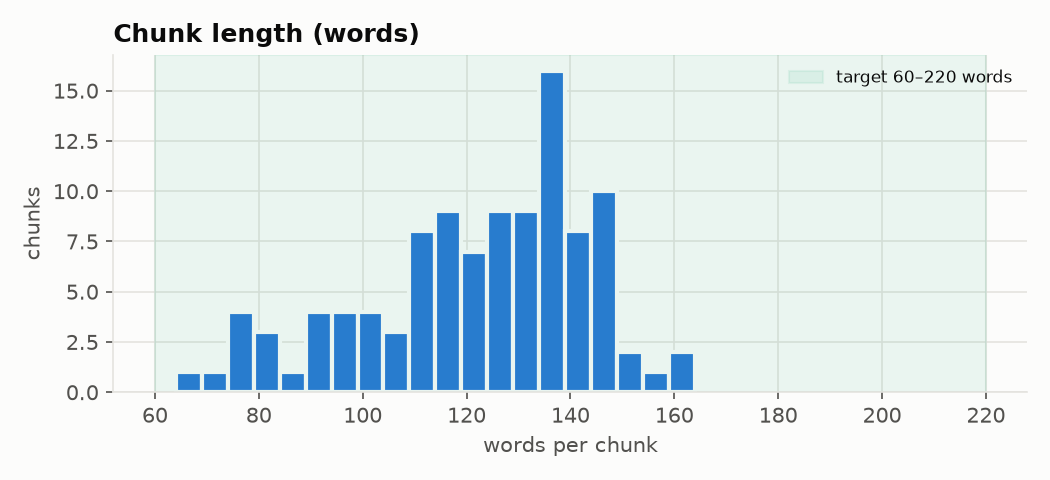
\includegraphics[width=0.49\columnwidth]{chunk_length_hist.png}\hfill
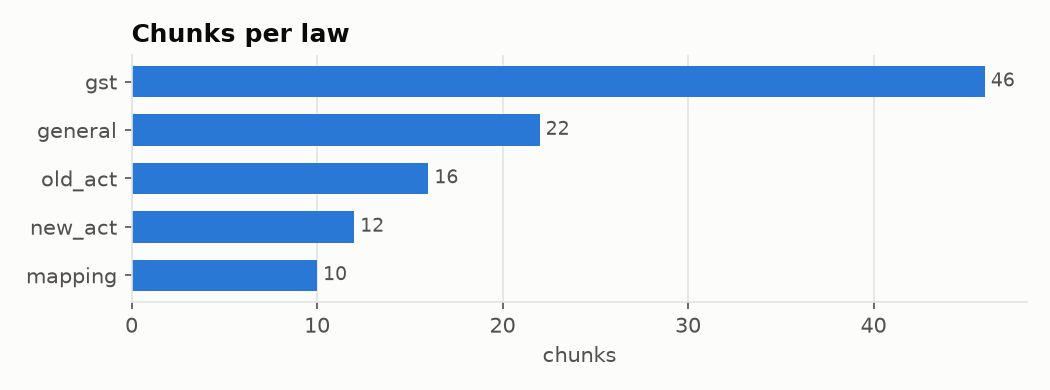
\includegraphics[width=0.49\columnwidth]{chunks_per_law.png}\\[2pt]
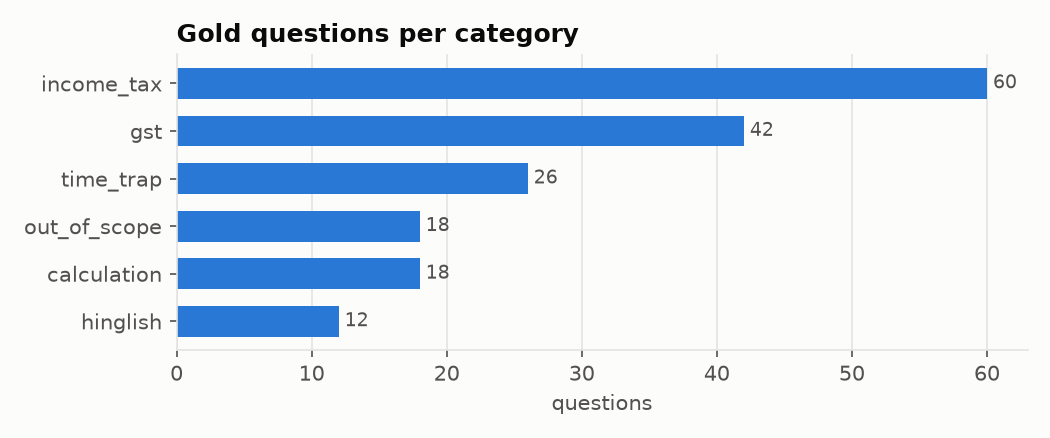
\includegraphics[width=0.49\columnwidth]{gold_categories.png}\hfill
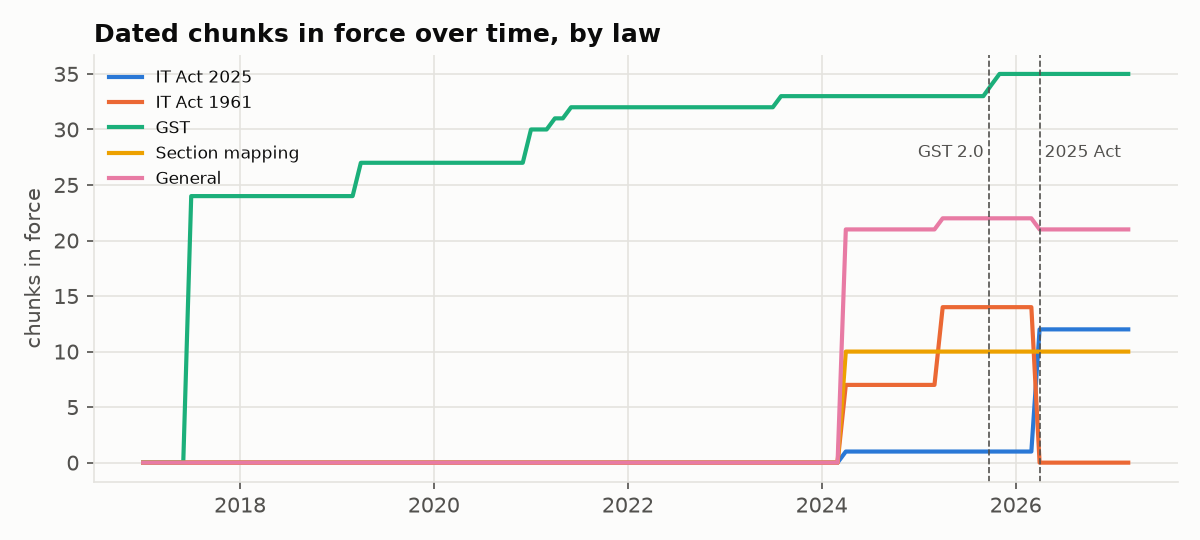
\includegraphics[width=0.49\columnwidth]{effective_date_coverage.png}
\caption{Exploratory analysis: chunk lengths, chunks per law, gold-set categories, and effective-date coverage.}
\label{fig:eda}
\end{figure}

\subsection{Temporal Metadata}
A chunk with \texttt{effective\_from} $f$ and \texttt{effective\_to} $t$ is eligible for a query period $[s,e]$ iff
\begin{equation}
f \le e \ \wedge\ (t = \varnothing \ \vee\ t \ge s),
\end{equation}
For example, new-regime slab passages exist in three versions (FY~2024-25, FY~2025-26, Tax Year~2026-27) and
each GST rate group has a pre- and post-22-September-2025 passage.

\subsection{Gold Set, Split and Leakage Control}
The 176 gold questions were written from the personas, not from the chunks: income tax 60, GST 42, time
traps 26, calculations 18, out-of-scope 18, Hinglish 12. Each row holds a reference answer, gold chunk IDs,
\emph{key facts} (short strings a correct answer must contain), category, language, difficulty and intent.
Time traps ask the same thing for different periods; calculation answers were hand-worked and cross-checked
against the calculator. There is no training on the knowledge base, but several choices \emph{are} tuned
(refusal threshold, number of passages, prompt wording, Hinglish dictionary). These were tuned on the 53-question
dev split only; the 123-question test split was run once, with the frozen final configuration. The intent
classifier's 356 training rows were written separately and checked to contain no gold or real question.

\subsection{Real-Question Set}
To check generalisation beyond team-written questions we collected 80 real questions from Reddit (36),
official FAQs (25), CAclubindia and other forums (12) and Quora (7), removed names and usernames, and
labelled coverage (full 51, partial 18, none 11). This set was never used for tuning.

% =====================================================================================
\section{System Architecture}

Taxot is a fixed pipeline: documents are indexed once, and every query passes the same steps and must clear
a guardrail gate before an answer is shown (Fig.~\ref{fig:arch}, Table~\ref{tab:steps}).

\begin{figure*}[t]
\centering
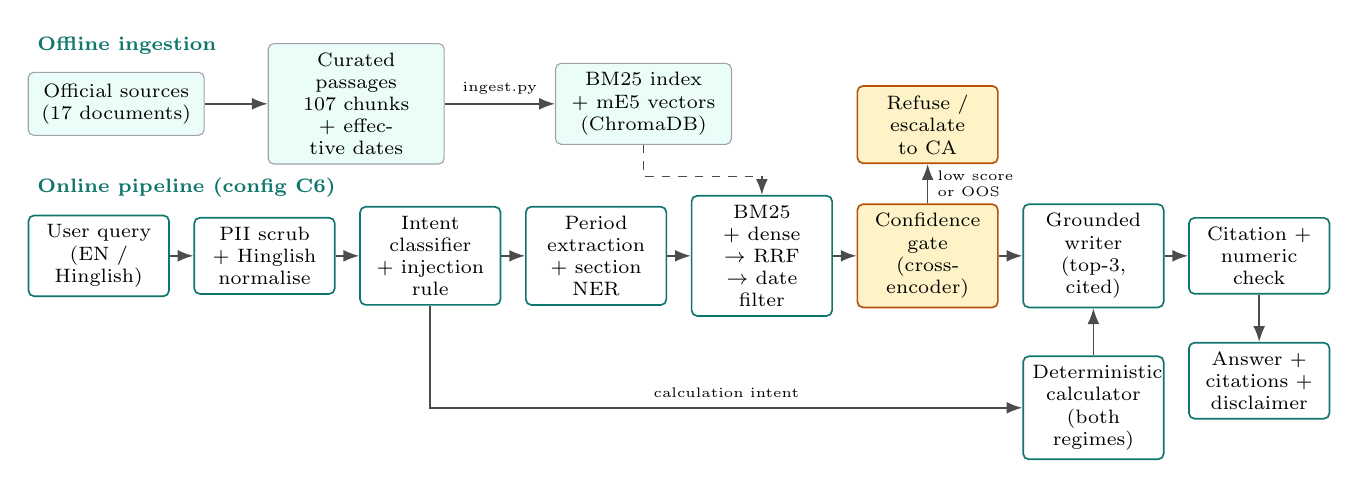
\begin{tikzpicture}[
  node distance=3mm and 3mm,
  stage/.style={draw=teal, fill=white, rounded corners=2pt, align=center, font=\scriptsize, minimum height=9mm, text width=15.5mm, line width=0.6pt},
  gate/.style={stage, draw=amber, fill=ambersoft},
  store/.style={draw=greybar, fill=tealsoft!40, rounded corners=2pt, align=center, font=\scriptsize, minimum height=8mm, text width=20mm},
  arr/.style={-{Latex[length=2mm]}, line width=0.6pt, draw=black!70},
  lbl/.style={font=\scriptsize\bfseries, text=teal}
]
% offline
\node[store] (src) {Official sources\\(17 documents)};
\node[store, right=8mm of src] (cur) {Curated passages\\107 chunks\\+ effective dates};
\node[store, right=14mm of cur] (idx) {BM25 index\\+ mE5 vectors\\(ChromaDB)};
\draw[arr] (src) -- (cur);
\draw[arr] (cur) -- node[above, font=\tiny]{ingest.py} (idx);
\node[lbl, above=1mm of src.north west, anchor=south west] {Offline ingestion};
% online
\node[stage, below=10mm of src.south west, anchor=north west] (q) {User query\\(EN / Hinglish)};
\node[stage, right=of q] (pii) {PII scrub\\+ Hinglish\\normalise};
\node[stage, right=of pii] (int) {Intent\\classifier\\+ injection rule};
\node[stage, right=of int] (per) {Period\\extraction\\+ section NER};
\node[stage, right=of per] (ret) {BM25 + dense\\$\rightarrow$ RRF\\$\rightarrow$ date filter};
\node[gate, right=of ret] (gate) {Confidence\\gate\\(cross-encoder)};
\node[stage, right=of gate] (gen) {Grounded\\writer\\(top-3, cited)};
\node[stage, right=of gen] (cit) {Citation +\\numeric\\check};
\node[stage, below=6mm of gen] (calc) {Deterministic\\calculator\\(both regimes)};
\node[gate, above=5mm of gate] (ref) {Refuse /\\escalate to CA};
\node[stage, below=6mm of cit] (out) {Answer +\\citations +\\disclaimer};
\draw[arr] (q) -- (pii); \draw[arr] (pii) -- (int); \draw[arr] (int) -- (per);
\draw[arr] (per) -- (ret); \draw[arr] (ret) -- (gate); \draw[arr] (gate) -- (gen);
\draw[arr] (gen) -- (cit); \draw[arr] (cit) -- (out);
\draw[arr] (gate) -- node[right, font=\tiny, align=left]{low score\\or OOS} (ref);
\draw[arr] (int.south) |- node[pos=0.75, above, font=\tiny]{calculation intent} (calc.west);
\draw[arr] (calc) -- (gen);
\draw[arr, dashed] (idx.south) -- ++(0,-4mm) -| (ret.north);
\node[lbl, above=1mm of q.north west, anchor=south west] {Online pipeline (config C6)};
\end{tikzpicture}
\caption{Taxot NLP architecture. Offline, curated passages with effective dates are indexed for BM25 and dense
retrieval. Online, every query passes the same steps; refusals happen only at the gate, and numbers come
only from the calculator.}
\label{fig:arch}
\end{figure*}

\begin{table}[t]
\caption{Pipeline Steps (Final Configuration C6)}
\label{tab:steps}
\centering
\footnotesize
\begin{tabular}{@{}p{0.22\columnwidth}p{0.70\columnwidth}@{}}
\toprule
Step & Implementation \\
\midrule
PII scrub & Regex for PAN, Aadhaar, phone, e-mail; masked before logging or any LLM call \\
Hinglish & Language detection + $\sim$150-entry dictionary (``kitna'', ``milta hai'', ``naye''); replacements shown in the trace \\
Intent & TF-IDF (word 1--2, char 2--5 grams) + logistic regression over question / calculation / out-of-scope; 356 rows, 5-fold CV accuracy 0.89; prompt-injection regex \\
Period & Rules for FY/AY/Tax Year, month-year, ``before GST 2.0'', ``last year''; default today, flagged \emph{assumed current law} \\
Sections & Regex (``80C'', ``u/s 44ADA'', ``115BAC'') $\to$ mapping-chunk boost (1961 $\leftrightarrow$ 2025) \\
Retrieval & BM25 + \texttt{multilingual-e5-small} $\to$ RRF ($k{=}60$) $\to$ date filter with period substitution $\to$ top 20 \\
Gate & \texttt{bge-reranker-base} scores top 20; refuse if intent is out-of-scope or best score $<\theta$ ($\theta{=}{-}5.83$, tuned on dev) \\
Calculator & Parse salary, deductions, age, tax year, currency $\to$ deterministic Python; follow-up question if inputs missing \\
Writer & Top-3 passages labelled \texttt{[CHUNK-ID]}; ``explain, don't compute''; Qwen2.5-3B (local) or hosted model via a gateway \\
Citation check & Each sentence must carry a valid retrieved ID; amounts must match calculator or passages; else extractive fallback \\
Output & Disclaimer, citations with effective dates, full JSON trace \\
\bottomrule
\end{tabular}
\end{table}

\textbf{Design decisions.} \emph{Hybrid retrieval}: BM25 catches exact tokens (section numbers, form names,
``August 2025''); dense embeddings catch paraphrase and Hinglish. \emph{Date filter before ranking}: only
chunks valid for the asked period are eligible; with no date, current law is used and the answer says so.
\emph{Calculator, never the LLM, for numbers}: slabs, rebates, surcharge and cess are deterministic rules.
\emph{Citation check}: we do not trust LLM citations~\cite{gao2023alce}; unsupported sentences are removed,
and if too little survives, an extractive answer built from the passages is returned.

% =====================================================================================
\section{Experimental Setup (M3)}

\subsection{Ablation Ladder}
Each configuration changes one thing (Table~\ref{tab:ladder}). Retrieval, refusal and calculator metrics
were computed for all configurations; LLM-answer metrics (about 25\,s per answer on CPU) for B0, B1, C2, C4
and C6, the configurations that mark each major step. All runs are logged to MLflow.

\begin{table}[t]
\caption{Ablation Ladder}
\label{tab:ladder}
\centering
\footnotesize
\begin{tabular}{@{}llcccc@{}}
\toprule
Cfg & Retrieval & Date & Hing. & Reranker & Gen. \\
\midrule
B0 & none (LLM alone) & -- & -- & -- & plain \\
B1 & BM25 top-5 & -- & -- & -- & grounded \\
C1 & dense (mE5) top-5 & -- & -- & -- & grounded \\
C2 & BM25 + dense, RRF & -- & -- & -- & grounded \\
C3 & C2 top-20 & -- & -- & reorder + gate & grounded \\
C4 & C3 & \checkmark & -- & reorder + gate & grounded \\
C5 & C4 & \checkmark & \checkmark & reorder + gate & grounded \\
C6 & C2 order & \checkmark & \checkmark & gate only & grounded \\
\bottomrule
\end{tabular}
\end{table}

\subsection{Metrics}
Let $G_q$ be the gold chunks of $q$ and $R_q^k$ the top-$k$ retrieved list (answerable questions only).
\begin{itemize}
\item \textbf{Recall@5} $=\frac{1}{|Q|}\sum_q |G_q\cap R_q^5|/|G_q|$; \textbf{MRR@10}; \textbf{nDCG@5} with binary
relevance~\cite{jarvelin2002ndcg}.
\item \textbf{Period accuracy} (time traps): the top-1 chunk is valid for the question's period.
\item \textbf{Refusal accuracy}: refused $\Leftrightarrow$ not answerable; also out-of-scope refusal rate and
false-refusal rate.
\item \textbf{Calculator exact match}: every gold key fact (each regime's total tax and the better regime)
appears in the calculator output.
\item \textbf{Key-fact accuracy}: share of answers that contain \emph{all} key facts after normalisation.
\item \textbf{Citation validity}: share of cited IDs that were among the passages shown to the writer.
\item \textbf{Faithfulness (proxy)}: share of answer sentences kept by the citation check; a CPU stand-in for
RAGAS faithfulness~\cite{es2024ragas}.
\item \textbf{Latency}: end-to-end wall-clock time, p50 and p95.
\end{itemize}

\subsection{Implementation}
The system is written in Python~3.12. BM25 uses \texttt{rank\_bm25}; dense retrieval uses
\texttt{multilingual-e5-small} vectors in ChromaDB; the gate uses \texttt{bge-reranker-base}; the intent model uses
scikit-learn. Answers are written by Qwen2.5-3B~\cite{qwen2024} via Ollama
(temperature 0) for the M3 runs, and a hosted writer (Groq \texttt{gpt-oss-20b} with fallbacks) for the
deployed system. The backend is FastAPI and experiments are tracked in MLflow. Retrieval runs on a 4-vCPU CPU-only server. The code base
has 246 automated tests, including 29 calculator tests with hand-worked cases.

% =====================================================================================
\section{Results}

\subsection{Development Set}
Table~\ref{tab:dev} gives the main ablation results on the 53-question dev set and Fig.~\ref{fig:kf} the
answer quality of each generated configuration.

\begin{table*}[t]
\caption{Ablation Results on the Development Set (53 Questions). Answer Metrics Use Qwen2.5-3B on CPU.}
\label{tab:dev}
\centering
\footnotesize
\setlength{\tabcolsep}{4pt}
\begin{tabular}{@{}lcccccccccc@{}}
\toprule
Config & Recall@5 & MRR@10 & nDCG@5 & Period acc. & Refusal acc. & False refusal & Key-fact acc. & Citation valid. & Faithful. & p50 (s) \\
\midrule
B0 & -- & -- & -- & -- & 0.906 & 0.000 & 0.104 & -- & -- & 1.4 \\
B1 & 0.812 & 0.730 & 0.708 & \textbf{1.000} & \textbf{0.981} & 0.021 & 0.646 & \textbf{1.000} & 0.987 & 15.4 \\
C1 & 0.875 & 0.680 & 0.710 & 0.750 & \textbf{0.981} & 0.021 & -- & -- & -- & -- \\
C2 & 0.839 & 0.755 & 0.748 & 0.875 & \textbf{0.981} & 0.021 & 0.604 & 0.990 & 0.993 & 47.0$^*$ \\
C3 & 0.804 & 0.656 & 0.647 & \textbf{1.000} & \textbf{0.981} & 0.021 & -- & -- & -- & -- \\
C4 & 0.861 & 0.695 & 0.705 & \textbf{1.000} & \textbf{0.981} & 0.021 & \textbf{0.688} & \textbf{1.000} & 0.971 & 17.4 \\
C5 & 0.861 & 0.709 & 0.716 & \textbf{1.000} & \textbf{0.981} & 0.021 & -- & -- & -- & -- \\
\textbf{C6} & \textbf{0.917} & \textbf{0.830} & \textbf{0.831} & \textbf{1.000} & \textbf{0.981} & 0.021 & \textbf{0.688} & \textbf{1.000} & \textbf{1.000} & 16.8 \\
\midrule
B0, hosted writer & -- & -- & -- & -- & -- & -- & 0.312 & -- & -- & 2.5 \\
C6, hosted writer & 0.917 & 0.830 & 0.831 & 1.000 & 0.981 & 0.021 & \textbf{0.792} & 1.000 & 1.000 & 8.1 \\
\bottomrule
\multicolumn{11}{@{}p{\textwidth}@{}}{\scriptsize $^*$C2's latency is inflated because it ran concurrently with another evaluation job. -- = not applicable or not run with the LLM. Hosted writer: Groq \texttt{gpt-oss-20b} with fallbacks, re-scored 26 Nov 2026; p95 18.3\,s.}
\end{tabular}
\end{table*}

\begin{figure}[t]
\centering
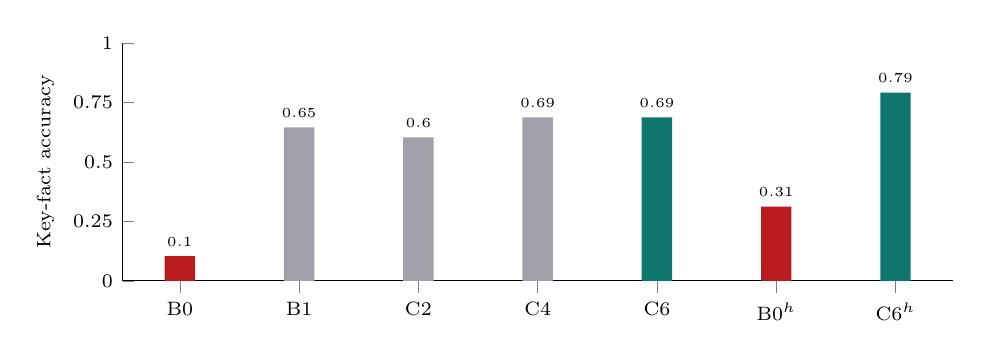
\begin{tikzpicture}
\begin{axis}[
  ybar, bar width=11pt, width=\columnwidth, height=4.6cm,
  ymin=0, ymax=1, ytick={0,0.25,0.5,0.75,1}, yticklabel style={font=\scriptsize},
  symbolic x coords={B0,B1,C2,C4,C6,B0h,C6h},
  xtick={B0,B1,C2,C4,C6,B0h,C6h}, xticklabels={B0,B1,C2,C4,C6,B0$^h$,C6$^h$},
  xticklabel style={font=\scriptsize},
  nodes near coords, nodes near coords style={font=\tiny, /pgf/number format/.cd, fixed, precision=2},
  ylabel={\scriptsize Key-fact accuracy}, axis lines*=left, enlarge x limits=0.08,
]
\addplot[fill=greybar, draw=none, bar shift=0pt] coordinates {(B1,0.646) (C2,0.604) (C4,0.688)};
\addplot[fill=redbar, draw=none, bar shift=0pt] coordinates {(B0,0.104) (B0h,0.312)};
\addplot[fill=teal, draw=none, bar shift=0pt] coordinates {(C6,0.688) (C6h,0.792)};
\end{axis}
\end{tikzpicture}
\caption{Key-fact accuracy on the dev set. The same LLM gets 10.4\% of key facts right alone (B0) and 68.8\%
inside Taxot (C6). $^h$: hosted writer.}
\label{fig:kf}
\end{figure}

\textbf{Retrieval is what makes the LLM useful.} The same Qwen2.5-3B answering from memory (B0) gets 10.4\% of
key facts right: it states pre-2025 rules (old slabs, the \rupee7~lakh rebate, 28\% GST on air conditioners)
and never cites. Grounded generation lifts this to 64.6\% with BM25 alone and 68.8\% in C6, with 100\%
citation validity. A larger hosted model remembers more (B0 31.2\%) but still cannot cite; inside Taxot it
reaches 79.2\%.

\textbf{Hybrid beats either retriever alone, but not on every metric.} Dense retrieval (C1) has higher
Recall@5 than BM25 (0.875 vs 0.812) but the worst period accuracy (0.75): embeddings treat ``GST on AC in
August 2025'' and ``GST on AC now'' as the same meaning. RRF fusion (C2) gives the best MRR among
single-stage systems.

\textbf{The reranker hurt when allowed to reorder.} C3 dropped MRR from 0.755 to 0.656.
\texttt{bge-reranker-base} supports English and Chinese only and often promotes a related passage or the
wrong period's version. Keeping the fusion order and using the cross-encoder only as the refusal signal (C6)
gave the best ranking overall. The multilingual \texttt{bge-reranker-v2-m3} took $\sim$25\,s per query on CPU.

\textbf{The date filter fixes time traps.} Period accuracy rises from 0.875 (C2) to 1.000 (C4) and stays there.

\textbf{Per category} (C6, Recall@5 / key-fact accuracy): income tax 0.92/0.50, GST 1.00/0.77, time traps
1.00/0.88, Hinglish 1.00/0.50, calculations 0.50/1.00. Long multi-fact income-tax answers and Hinglish answers
are the weakest: the 3B writer paraphrases numbers or omits one of several required facts. Calculation
questions often retrieve old-regime passages rather than rebate passages, but the calculator answer is exact.

\subsection{Held-Out Test Set}
\label{sec:test}
After all tuning was frozen, the test split (123 questions) was run once.
Table~\ref{tab:test} reports retrieval, refusal and calculator metrics for every configuration.
Answer metrics (key facts, citations) require LLM generation for every question and configuration; on
free-tier providers this was not feasible within the project, so they are reported on dev only.

\begin{table}[t]
\caption{Held-Out Test Set (123 Questions), Retrieval and Refusal}
\label{tab:test}
\centering
\footnotesize
\setlength{\tabcolsep}{3.5pt}
\begin{tabular}{@{}lcccccc@{}}
\toprule
Cfg & R@5 & MRR & nDCG@5 & Period & Refusal & Calc. \\
\midrule
\TestRows
\bottomrule
\end{tabular}
\end{table}

\TestDiscussion

\subsection{Real-World Check}
On the 80 real questions, the knowledge base fully covers 64\%, partly 23\% and not at all 14\%. On the 51
fully covered questions, C6 reaches Recall@5 0.62 by exact passage and 0.78 at rule level (any period
version of the gold rule). Most of the gap is temporal: posts written in 2025 were labelled with FY~2025-26
passages, while C6 deliberately answers with the law in force today. Real out-of-scope questions are harder
than synthetic ones: only 57\% (4/7) were refused. The most common real confusion (``no tax up to \rupee12 lakh
but 5\% from \rupee4 lakh?'', 10 posts) exposed a knowledge gap that we closed with an explainer passage.

% =====================================================================================
\section{Error Analysis and Improvement Iterations (M4)}

\subsection{Error Categories}
Labelling every dev failure of C6 with the M4 taxonomy gives: (a)~\emph{unsupported or incomplete claim}---the
writer paraphrased away a required number or dropped one of several facts (the largest category, mostly
income-tax and Hinglish answers); (b)~\emph{retrieval miss}---calculation questions retrieving old-regime
rather than rebate passages, and regime-switching or filing-procedure questions phrased very differently
from our passages; (c)~\emph{wrong refusal}---one false refusal out of 48 answerable questions;
(d)~\emph{wrong period}---none after the date filter; (e)~\emph{calculation-parsing error}---none on the gold
set, but several on real questions (below).

\subsection{Improvement Iterations}
\begin{enumerate}
\item \textbf{Reranker as gate, not ranker (C3$\to$C6).} MRR 0.656 $\to$ 0.830, Recall@5 0.804 $\to$ 0.917.
\item \textbf{Date filter with period substitution (C2$\to$C4/C6).} Period accuracy 0.875 $\to$ 1.000; when a
passage is from the wrong period, the same rule's in-period version replaces it, and questions about years
before our sources keep the closest version instead of returning nothing.
\item \textbf{Hosted writer behind a provider gateway.} Key-fact accuracy 68.8\% $\to$ 79.2\%, median latency
16.8\,s $\to$ 8.1\,s, citation validity unchanged at 1.00.
\item \textbf{Fixes from real questions.} Currency and per-month amount parsing, freelancer income under
s.~44ADA (s.~58 of the 2025 Act), calculator-only verdicts, removal of filler text, and the
\rupee12-lakh explainer passage; each was regression-tested on dev with no metric drop.
\end{enumerate}

\subsection{Robustness}
A battery of the 80 real questions plus 28 hand-written hard cases (foreign-currency income, per-month pay,
``CTC 18 LPA'', pensions, Hinglish such as ``meri salary 1 lakh mahina hai kitna tax lagega'', typos such as
``salry 15 lakh'', presumptive-limit edge cases) checks intent, parsed calculator inputs, follow-ups and
refusals with the writer switched off. \RobustText{} Prompt-injection attempts (``ignore your rules and
\ldots'') are caught by the injection rule before retrieval and refused. Hinglish/English pairs of the same
question retrieve the same gold chunks on dev (Hinglish Recall@5 1.00), and old section numbers (``80C'')
are bridged by the mapping chunks.

% =====================================================================================
\section{Deployment Prototype (M5)}

\textbf{Application.} A FastAPI service exposes \texttt{/ask} (question $\to$ answer, citations, trace),
\texttt{/compare} (plain LLM vs Taxot), \texttt{/calculate} (regime comparison), \texttt{/feedback},
\texttt{/experiments}, \texttt{/kb/stats} and \texttt{/health}, which reports the reachability of each LLM provider.
A static web front end (no build step) has Ask, Plain-LLM-vs-Taxot, Calculator, Tasks, Experiments and
Monitor and How-it-works tabs, a citations panel with effective dates, and thumbs-up/down feedback.

\textbf{Deployment.} The service is containerised (Dockerfile with models and indexes built into the image,
health check, API keys passed at run time) and runs as a \texttt{systemd} service on a 4-vCPU VPS.

\textbf{Performance.} \PerfText{}

\textbf{Monitoring.} Every query is logged (PII-scrubbed) with latency, intent, refusal flag and reason,
the gate's top score and the cited IDs; feedback votes and every LLM call (provider, model, latency, tokens)
are logged as JSON lines. A Monitor tab in the app (\texttt{GET /monitoring}) turns these logs into a dashboard:
questions per day with the refused share, refusal reasons, p50/p95 latency, thumbs-up share, recent thumbs-down,
answered questions whose gate score was within 1.0 of the threshold (likely knowledge-base gaps), and per-provider
LLM calls, success rate, latency and tokens. The real-question check found the \rupee12-lakh gap this way.

\textbf{Failure handling.} LLM timeout or rate limit $\to$ fall back to the next provider, then to the
extractive answer; no passage above threshold $\to$ refuse and suggest a CA; missing calculator inputs
$\to$ a follow-up question; presumptive-limit cases $\to$ escalation; a disclaimer on every answer.

% =====================================================================================
\section{Agentic Extension}

The pipeline answers one question with fixed steps; users' real jobs are longer (``check my Form~16 against
my AIS'', ``which ITR form and regime, and what next'', ``how can I save tax this year''). We therefore reused
the NLP pipeline as one tool (\texttt{search\_tax\_law}) inside a LangGraph orchestrator with a document agent,
income-tax, GST and calculator specialists, an escalation step that writes a CA summary, and a verifier from
a different model family. Every figure is computed by the unit-tested calculator and reconciled with code;
the user approves key steps; document text is treated as data, never as instructions.

On 59 synthetic tasks (40 fictitious taxpayers with generated Form~16, AIS and interest certificates, 21 with
planted problems and 4 with prompt injections) the system met all five targets: task success 100\%, tool-call
accuracy 100\%, verifier catch rate 100\% on 19 planted unsupported claims, correct escalation 100\% and
injection resistance 100\%. On the same 22 filing and tax-saving tasks, the NLP pipeline succeeds on 4.5\%
and a single agent with all tools on 45\% (Table~\ref{tab:agents}); the single agent picks the right form and
regime but fills the calculator itself and drops deductions. Without the verifier, 33 of 229 draft claims
(14\%) would have reached the user unsupported.

\begin{table}[t]
\caption{Tasks vs Answers: Same 22 Filing and Tax-Saving Tasks}
\label{tab:agents}
\centering
\footnotesize
\setlength{\tabcolsep}{3pt}
\begin{tabular}{@{}lccccc@{}}
\toprule
System & Success & Tax & Escal. & Calls & Med.\,s \\
\midrule
NLP pipeline (decomp.) & 4.5\% & 56\% & 73\% & 0 & 12 \\
Single agent, all tools & 45\% & 58\% & 89\% & 7.1 & 66 \\
\textbf{Multi-agent Taxot} & \textbf{100\%} & \textbf{100\%} & \textbf{100\%} & 19.8 & 244 \\
\bottomrule
\end{tabular}
\end{table}

% =====================================================================================
\section{Limitations and Ethics}

\begin{itemize}
\item \textbf{Curated summaries, not full Acts.} 35 of 107 chunks are checked only against secondary
sources; a summary can omit a proviso that matters to a user.
\item \textbf{Gold set authored by the team} and not reviewed by a CA; the same people wrote the corpus and the
questions, which may inflate retrieval scores. The dev set is small (53), so differences of a few points are
within noise.
\item \textbf{Out-of-scope refusal on test} is 84.6\% (target 90\%), and only 57\% on real questions: enforcement and evasion
questions that look like ordinary GST questions pass the classifier.
\item \textbf{Latency target missed.} The 5\,s median needs a faster writer; the hosted writer gives 8.1\,s.
\item \textbf{English-centric reranker}; the multilingual reranker was too slow on CPU.
\item \textbf{Rule-based period extraction} covers common patterns; anything else falls back to ``assumed current
law'', which is shown to the user.
\item \textbf{Calculator scope}: individuals, both regimes, FY~2024-25 to Tax Year~2026-27, salary and presumptive
income; no capital-gains computation.
\item \textbf{Free-tier LLMs} see only masked text, but providers may log requests; evaluation used synthetic
and public data only.
\item \textbf{Liability.} Taxot is informational and not affiliated with the Income Tax Department; every answer
carries a disclaimer, and notices, disputes and evasion requests are refused with a CA referral.
\end{itemize}

% =====================================================================================
\section{Conclusion and Future Work}

Taxot shows that, for a domain whose answers change with the date, the components around the LLM decide
quality: hybrid retrieval with an explicit period filter, a gate that knows when to abstain, a calculator for
every number, and a citation check that does not trust the model. The same 3B model goes from 10\% to 69\% of
key facts right with every citation valid. Of the five targets fixed before building, four are met on the dev set;
on the held-out test set, retrieval and the calculator hold up, but out-of-scope refusal (84.6\%) and latency miss their
targets.
Future work: more enforcement and evasion examples for the out-of-scope classifier, validated on fresh questions; CA review of 30--50 gold answers, LLM-judge faithfulness and test-set answer metrics, a faster or
GPU-served writer to meet the 5\,s target, a quantised multilingual reranker, full-text Act ingestion, and a
user study with the three personas.

% =====================================================================================
\begin{thebibliography}{99}
\footnotesize
\bibitem{zhang2021situatedqa} M. J. Q. Zhang and E. Choi, ``SituatedQA: Incorporating extra-linguistic contexts into QA,'' in \emph{Proc. EMNLP}, 2021, pp. 7371--7387.
\bibitem{chen2021timeqa} W. Chen, X. Wang, and W. Y. Wang, ``A dataset for answering time-sensitive questions,'' in \emph{Proc. NeurIPS Datasets and Benchmarks}, 2021.
\bibitem{magesh2025hallucination} V. Magesh, F. Surani, M. Dahl, M. Suzgun, C. D. Manning, and D. E. Ho, ``Hallucination-free? Assessing the reliability of leading AI legal research tools,'' \emph{J. Empirical Legal Studies}, vol. 22, no. 2, 2025.
\bibitem{khanuja2020gluecos} S. Khanuja, S. Dandapat, A. Srinivasan, S. Sitaram, and M. Choudhury, ``GLUECoS: An evaluation benchmark for code-switched NLP,'' in \emph{Proc. ACL}, 2020, pp. 3575--3585.
\bibitem{robertson2009bm25} S. Robertson and H. Zaragoza, ``The probabilistic relevance framework: BM25 and beyond,'' \emph{Found. Trends Inf. Retr.}, vol. 3, no. 4, pp. 333--389, 2009.
\bibitem{karpukhin2020dpr} V. Karpukhin \emph{et al.}, ``Dense passage retrieval for open-domain question answering,'' in \emph{Proc. EMNLP}, 2020, pp. 6769--6781.
\bibitem{wang2022e5} L. Wang \emph{et al.}, ``Text embeddings by weakly-supervised contrastive pre-training,'' arXiv:2212.03533, 2022.
\bibitem{wang2024me5} L. Wang \emph{et al.}, ``Multilingual E5 text embeddings: A technical report,'' arXiv:2402.05672, 2024.
\bibitem{chen2024m3} J. Chen, S. Xiao, P. Zhang, K. Luo, D. Lian, and Z. Liu, ``M3-Embedding: Multi-linguality, multi-functionality, multi-granularity text embeddings through self-knowledge distillation,'' in \emph{Findings of ACL}, 2024.
\bibitem{cormack2009rrf} G. V. Cormack, C. L. A. Clarke, and S. Buettcher, ``Reciprocal rank fusion outperforms Condorcet and individual rank learning methods,'' in \emph{Proc. SIGIR}, 2009, pp. 758--759.
\bibitem{nogueira2019passage} R. Nogueira and K. Cho, ``Passage re-ranking with BERT,'' arXiv:1901.04085, 2019.
\bibitem{lewis2020rag} P. Lewis \emph{et al.}, ``Retrieval-augmented generation for knowledge-intensive NLP tasks,'' in \emph{Proc. NeurIPS}, 2020.
\bibitem{gao2023alce} T. Gao, H. Yen, J. Yu, and D. Chen, ``Enabling large language models to generate text with citations,'' in \emph{Proc. EMNLP}, 2023.
\bibitem{liu2023verifiability} N. F. Liu, T. Zhang, and P. Liang, ``Evaluating verifiability in generative search engines,'' in \emph{Findings of EMNLP}, 2023.
\bibitem{es2024ragas} S. Es, J. James, L. Espinosa-Anke, and S. Schockaert, ``RAGAS: Automated evaluation of retrieval augmented generation,'' in \emph{Proc. EACL (Demos)}, 2024.
\bibitem{zheng2021casehold} L. Zheng, N. Guha, B. R. Anderson, P. Henderson, and D. E. Ho, ``When does pretraining help? Assessing self-supervised learning for law and the CaseHOLD dataset,'' in \emph{Proc. ICAIL}, 2021.
\bibitem{malik2021ildc} V. Malik \emph{et al.}, ``ILDC for CJPE: Indian legal documents corpus for court judgment prediction and explanation,'' in \emph{Proc. ACL-IJCNLP}, 2021.
\bibitem{pipitone2024legalbenchrag} N. Pipitone and G. Houir Alami, ``LegalBench-RAG: A benchmark for retrieval-augmented generation in the legal domain,'' arXiv:2408.10343, 2024.
\bibitem{aguilar2020lince} G. Aguilar, S. Kar, and T. Solorio, ``LinCE: A centralized benchmark for linguistic code-switching evaluation,'' in \emph{Proc. LREC}, 2020.
\bibitem{kamath2020selective} A. Kamath, R. Jia, and P. Liang, ``Selective question answering under domain shift,'' in \emph{Proc. ACL}, 2020.
\bibitem{gao2023pal} L. Gao \emph{et al.}, ``PAL: Program-aided language models,'' in \emph{Proc. ICML}, 2023.
\bibitem{schick2023toolformer} T. Schick \emph{et al.}, ``Toolformer: Language models can teach themselves to use tools,'' in \emph{Proc. NeurIPS}, 2023.
\bibitem{yao2023react} S. Yao \emph{et al.}, ``ReAct: Synergizing reasoning and acting in language models,'' in \emph{Proc. ICLR}, 2023.
\bibitem{jarvelin2002ndcg} K. J\"arvelin and J. Kek\"al\"ainen, ``Cumulated gain-based evaluation of IR techniques,'' \emph{ACM Trans. Inf. Syst.}, vol. 20, no. 4, pp. 422--446, 2002.
\bibitem{qwen2024} Qwen Team, ``Qwen2.5 technical report,'' arXiv:2412.15115, 2024.
\end{thebibliography}

\end{document}
